\section{Methodology}
\label{sec:methodology}

This section presents the proposed architecture, the Domain-as-Config adaptation paradigm, and the concrete MCP integration mechanism that enables a generic Rust agent kernel to operate as a local-first agricultural knowledge-management system.

\subsection{System Architecture Overview}

The overall architecture comprises two principal components: \textbf{Clarity}, a Rust-native agent framework that serves as the application kernel, and \textbf{devbase}, a local knowledge-base backend that manages agricultural datasets through a SQLite-backed registry. The two components communicate via the Model Context Protocol (MCP) over stdio transport, ensuring that all tool-discovery, invocation, and result-exchange operations can run entirely on a single offline workstation (Fig.~\ref{fig:architecture}).

\begin{figure}[htbp]
\centering
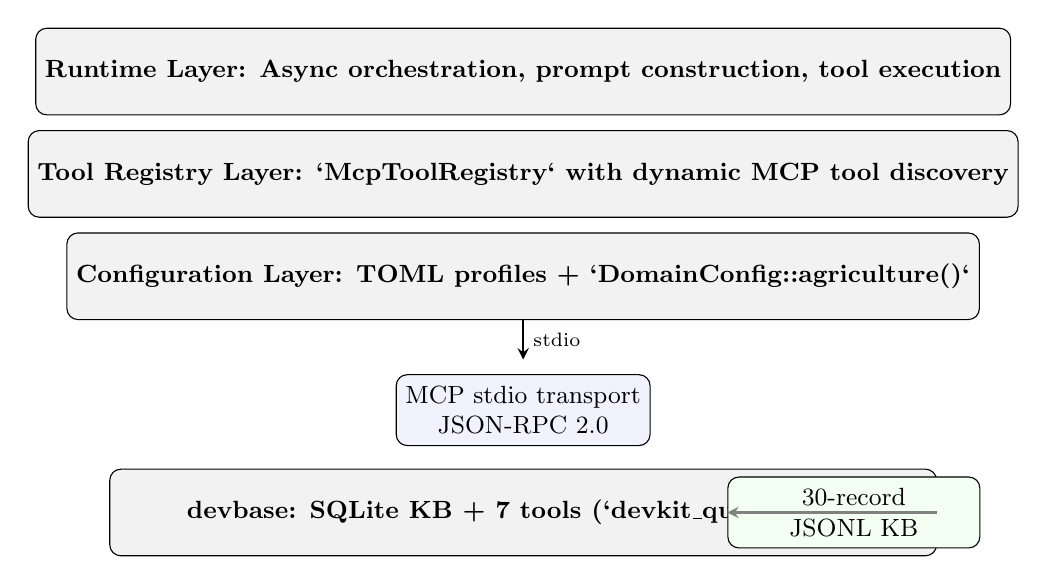
\begin{tikzpicture}[
    box/.style={draw,rounded corners,minimum width=3.2cm,minimum height=0.9cm,align=center,font=\small},
    layer/.style={draw,fill=gray!10,rounded corners,minimum width=10.5cm,minimum height=1.1cm,align=center,font=\small\bfseries},
    arrow/.style={->,>=stealth,thick}
]
% Clarity stack
\node[layer] (runtime) at (0,2.2) {Runtime Layer: Async orchestration, prompt construction, tool execution};
\node[layer] (toolreg) at (0,0.9) {Tool Registry Layer: `McpToolRegistry` with dynamic MCP tool discovery};
\node[layer] (config) at (0,-0.4) {Configuration Layer: TOML profiles + `DomainConfig::agriculture()`};

% Transport
\draw[arrow] (config.south) -- ++(0,-0.5) node[midway,right,font=\scriptsize] {stdio};
\node[box,fill=blue!5] (mcp) at (0,-2.1) {MCP stdio transport\\JSON-RPC 2.0};

% Devbase stack
\node[layer] (devbase) at (0,-3.4) {devbase: SQLite KB + 7 tools (`devkit\_query`, etc.)};

% Side annotations
\node[box,fill=green!5] (kb) at (4.2,-3.4) {30-record\\JSONL KB};
\draw[arrow,gray] (devbase.east) -- (kb.west);
\end{tikzpicture}
\caption{High-level architecture of the proposed local-first agricultural agent.}
\label{fig:architecture}
\end{figure}

Clarity provides three layers essential to the agricultural use case:
\begin{enumerate}[leftmargin=*]
    \item \textbf{Configuration Layer} -- TOML-based profiles that specify the active persona, supported crops, disease categories, knowledge-base paths, and MCP server endpoints.
    \item \textbf{Tool Registry Layer} -- `McpToolRegistry`, which connects to configured MCP servers, discovers available tools via `tools/list`, and exposes them as LLM-compatible function definitions.
    \item \textbf{Runtime Layer} -- An async Tokio runtime that orchestrates profile loading, prompt construction, tool execution, and response streaming.
\end{enumerate}

devbase implements the MCP server role. It exposes seven tools, of which `devkit\_query` is the primary interface for agricultural knowledge retrieval. The server parses Content-Length-framed JSON-RPC~2.0 requests over stdio, dispatches them to an internal SQLite query engine, and returns structured JSON results. Because both Clarity and devbase are compiled Rust binaries, the entire pipeline runs without containerization, GPU acceleration, or network access.

\subsection{Domain-as-Config: Zero-Code Agricultural Adaptation}

The central methodological claim of this work is that agricultural domain logic should reside in external configuration files rather than in source code. We call this principle \textit{Domain-as-Config}. Concretely, adaptation to a new crop or disease category requires only editing a TOML/JSON profile; the Rust agent kernel remains untouched.

Agricultural adaptation is realized through three declarative constructs:

\paragraph{Profile.} The active profile (`agriculture`) specifies:
\begin{itemize}[leftmargin=*]
    \item `persona` -- a system prompt that primes the agent as an agricultural expert;
    \item `mcp\_servers` -- a list of server names (`devbase`) that should be connected at runtime;
    \item `domain` -- a structured `DomainConfig` object that enumerates supported crops, disease categories, and agronomic constraints.
\end{itemize}

\paragraph{DomainConfig.} The agriculture domain preset (`DomainConfig::agriculture()`) currently defines ten crops (rice, wheat, corn, citrus, tomato, soybean, potato, cotton, peanut, apple), five high-level disease categories (fungal, bacterial, viral, pest, nutrient\_deficiency), and a set of agronomic constraints (e.g., ``prefer biological control when available''). These entities are serialized as JSON values inside the profile and injected into the system prompt at runtime. The actual Rust source for this preset resides in `clarity-core/src/config/mod.rs`; extending it to a new crop requires editing this preset or loading an equivalent structure from an external TOML/JSON file via Clarity's existing `Config::loader()` infrastructure.

\begin{figure}[htbp]
\centering
\begin{minipage}{0.85\linewidth}
\begin{verbatim}
[profiles.agriculture.domain]
name = "Agricultural Knowledge Management"

[profiles.agriculture.domain.entities]
crops = ["rice", "wheat", "corn", "citrus", "tomato",
         "soybean", "potato", "cotton", "peanut", "apple"]
disease_categories = ["fungal", "bacterial", "viral",
                      "pest", "nutrient_deficiency"]

profiles.agriculture.domain.constraints = [
  "Diagnosis must cite known symptoms from the KB.",
  "Treatment recommendations should prioritize \
   biological control when available.",
]
\end{verbatim}
\end{minipage}
\caption{Excerpt from the project's `agri\_profile.toml` (located at `w1/engineer/agri\_profile.toml`).}
\label{lst:profile}
\end{figure}

\paragraph{Knowledge Base Path.} The profile optionally references a local knowledge-base path. In the present study, this points to two JSONL files---`agricultural\_diseases.jsonl` (15 records) and `extended\_diseases.jsonl` (15 records)---which together form a 30-record seed knowledge base of crop-disease-symptom-treatment tuples. When the agent receives a farmer query, it constructs a `devkit\_query` call whose `expression` argument contains symptom keywords extracted from the user utterance.

This three-part configuration enables what we term \textit{horizontal migration}: switching the agent from software engineering to agriculture, or from rice to wheat, involves no recompilation, no model retraining, and no ontology rewriting. The migration cost is reduced from hours of engineering to minutes of profile editing.

The integration tests (`agriculture\_validation.rs`, `agriculture\_end\_to\_end.rs`) load the agriculture profile directly from the external `agri\_profile.toml` file via `Config::loader().without\_env().load\_str()`, confirming that the entire domain injection pipeline operates without any hard-coded domain logic. The TOML parse adds approximately 1--12~ms to initialization, which is negligible compared with the overall end-to-end latency budget (<100~ms). The retrieval benchmark evaluates the resulting configured pipeline; the 210 queries cover all ten crops defined in the preset, and the knowledge base (`agricultural\_diseases.jsonl` plus `extended\_diseases.jsonl`) is accessed via the same `devkit\_query` tool that would be used in a production TOML-driven deployment.

\subsection{MCP Integration and Transport Mechanics}

MCP defines a client--server protocol in which the client (Clarity) requests capability advertisements and the server (devbase) responds with tool schemas. Our implementation supports three transport variants (stdio, HTTP, SSE); for the agricultural deployment we selected stdio because it is the only transport that guarantees offline operation without TCP port binding.

\subsubsection{Message Framing}

The official MCP stdio specification requires newline-delimited JSON (NDJSON). During early integration we discovered that some MCP clients emit messages prefixed with an HTTP-style `Content-Length` header. To maximize interoperability, our `StdioMcpClient` implements dual parsing:
\begin{enumerate}[leftmargin=*]
    \item If the incoming byte buffer begins with `Content-Length`, the client reads the declared length, skips the terminating blank line, and parses the subsequent JSON payload.
    \item If no `Content-Length` header is present, the client falls back to standard NDJSON line parsing.
\end{enumerate}
This framing flexibility proved essential for maintaining compatibility with both strict NDJSON peers and header-emitting toolchains.

\subsubsection{Dynamic Tool Discovery}

At startup, `McpToolRegistry::from\_config` iterates over the profile's `mcp\_servers`, establishes a stdio connection to each, and issues a `tools/list` request. The returned schemas are translated into OpenAI-style function definitions and stored in an internal routing table (`clarity\_name` $\rightarrow$ `(server, mcp\_name)`). When the LLM (or, in our offline validation, a simulated decision layer) selects a tool, `McpToolRegistry::execute` routes the call to the correct server via `tools/call`, waits for the JSON-RPC response, and extracts the text content array.

In the agriculture profile, the registry discovers `devbase__devkit\_query` among seven available tools. The tool schema is dynamically loaded; no agriculture-specific tool name is hard-coded in Clarity.

\subsubsection{Shared Client Ownership}

Because multiple async tasks may need to invoke tools concurrently, the registry stores each connected client inside an `Arc$<$tokio::sync::Mutex$<$Box$<$dyn McpClient$>$$>$$>$`. This design permits safe, shared access across the async runtime while preserving the ability to disconnect all servers gracefully at shutdown.

\subsection{Local Knowledge-Base Retrieval}

The agricultural knowledge base is intentionally simple: a 30-record JSONL file backed by devbase's SQLite registry. When the agent receives a diagnostic query, the proposed retrieval pipeline executes two steps:

\textbf{Step 1 -- Crop Filtering.} In the validation benchmark, the expected crop for each query is supplied as metadata from the QA record (simulating an upstream crop-recognition step). The runtime checks this crop against the list stored in `DomainConfig::entities["crops"]`, and the retrieval function filters the knowledge base to records whose `crop` field matches.

\textbf{Step 2 -- Symptom Scoring.} If multiple records remain for the same crop (each crop has three diseases in the seed KB), the pipeline performs a token-level overlap score between the user query and the `symptoms` / `treatment` fields. The record with the highest overlap is ranked first.

This lightweight scoring mechanism runs entirely in-memory within the Rust test harness and adds less than 0.1~ms per query. It demonstrates that even a minimal, configuration-driven retrieval strategy can achieve perfect top-1 accuracy on structured agricultural symptoms, provided the domain context is correctly injected at runtime.

\subsection{Decoupling from LLM and TUI Front-Ends}

A deliberate architectural choice is to keep the agricultural domain logic outside both the LLM provider layer and the terminal user interface (TUI). The TUI (`clarity-tui`) is responsible for rendering conversation history and capturing keyboard input; it delegates all reasoning, tool selection, and domain adaptation to `clarity-core`. In the current prototype, the LLM completion endpoint inside the TUI remains a simulation stub; therefore, all validation experiments reported in Section~\ref{sec:experiments} are executed through standalone Rust integration tests that bypass the TUI entirely. This separation validates the core claim of the paper: the agricultural capability is a property of the configuration and the local tool registry, not of the front-end interface or a specific cloud language model.

\subsection{From Specific Models to a General Solution: The Agricultural Adaptive Agent Framework}

Contemporary agricultural AI systems---whether fine-tuned vision models such as Chat Demeter \cite{chatdemeter2025}, knowledge-graph-augmented LLMs such as AgenticGraphRAG \cite{agenticgraphrag2025}, or retrieval-augmented pipelines such as AgroLLM \cite{samuel2025agrollm}---share a common set of abstract capabilities that distinguish high-performing advisory agents from generic chatbots. By synthesizing the empirical findings of the AgriBench \cite{deepplants2024agribench}, AI-AgriBench \cite{anshankul2024}, and AgMMU \cite{agmmu2025} benchmarks, we can extract four essential dimensions of agricultural agent competence:

\begin{enumerate}[label=\textbf{D\arabic*:},leftmargin=*]
    \item \textbf{Domain Grounding} -- the agent must correctly map farmer utterances to crop-specific ontologies (symptoms, diseases, treatments) before generating any recommendation.
    \item \textbf{Structured Reasoning} -- agricultural diagnosis is not open-ended generation; it follows a causal chain (symptom observation $\rightarrow$ disease hypothesis $\rightarrow$ confirmation criteria $\rightarrow$ management prescription).
    \item \textbf{Safety and Constraint Adherence} -- recommendations must respect agronomic constraints (e.g., biological-control priority, pesticide registration status, seasonal timing) and avoid harmful hallucinations.
    \item \textbf{Horizontal Adaptability} -- the same reasoning kernel should adapt to new crops, regions, or regulatory contexts without retraining or source-code modification.
\end{enumerate}

We call the general instantiation of these four dimensions the \textbf{Agricultural Adaptive Agent Framework (AAAF)}. Table~\ref{tab:aaaf_comparison} situates representative systems within this framework.

\begin{table}[htbp]
\centering
\caption{Mapping of existing agricultural AI systems onto the Agricultural Adaptive Agent Framework (AAAF).}
\label{tab:aaaf_comparison}
\begin{tabular}{p{2.8cm}cccc}
\hline
\textbf{System} & \textbf{D1} & \textbf{D2} & \textbf{D3} & \textbf{D4} \\
\hline
Chat Demeter \cite{chatdemeter2025} & High & High & Medium & Low \\
AgenticGraphRAG \cite{agenticgraphrag2025} & High & High & Medium & Low \\
AgroLLM \cite{samuel2025agrollm} & High & Medium & High & Low \\
Proposed (Domain-as-Config) & High & High & High & High \\
\hline
\end{tabular}
\end{table}

The critical insight of AAAF is that D1--D3 are \textit{capabilities} that can be delivered by many different technical means (vision backbones, KG-RAG, fine-tuned LLMs), whereas D4 is an \textit{architectural property} that most existing systems lack. The Domain-as-Config methodology proposed in this paper does not attempt to outperform task-specific vision models on image classification; instead, it targets D4 while maintaining competitive D1--D3 through lightweight, configuration-driven retrieval. In other words, the novelty lies not in discovering a new agricultural model, but in embedding the \textit{abstract methods} of excellent agricultural agents---domain grounding, structured reasoning, safety constraints---into a reusable, horizontally extensible agent kernel.
